\PassOptionsToPackage{utf8}{inputenc}
\documentclass{bioinfo}
\copyrightyear{2017} \pubyear{2017}

\access{Advance Access Publication Date: Day Month Year}
\appnotes{Original Article}

\begin{document}
\firstpage{1}

\subtitle{Genome Analysis}

\title[Dryhic]{OneD: increasing reproducibility of Hi-C Samples with abnormal karyotypes}

\author[Vidal \textit{et~al}.]{Enrique Vidal\,$^{\text{\sfb 1,2}*}$, François le Dily\,$^{\text{\sfb 1,2}}$, Javier Quilez\,$^{\text{\sfb 1,2}}$, Ralph Stadhouders\,$^{\text{\sfb 1,2}}$, Yasmina Cuartero\,$^{\text{\sfb 1,2}}$,Miguel Beato\,$^{\text{\sfb 1,2}}$ and Guillaume Fillion\,$^{\text{\sfb 1,2}}$}

\address{$^{\text{\sf 1}}$Gene Regulation, Stem Cells and Cancer Program, Centre for Genomic Regulation (CRG), The
	Barcelona Institute of Science and Technology (BIST), Barcelona, Spain \\
	$^{\text{\sf 2}}$Universitat Pompeu Fabra (UPF), Barcelona, Spain}

\corresp{$^\ast$To whom correspondence should be addressed.}

\history{Received on XXXXX; revised on XXXXX; accepted on XXXXX}

\editor{Associate Editor: XXXXXXX}

\abstract{
  \textbf{Motivation:} The three-dimensional conformation of genomes is an
essential component of their biological activity. The advent of the Hi-C
technology enabled an unprecedented advance in our understanding of genome
structures. However, Hi-C is subject to systematic biases that can
compromise downstream analyses. Several strategies have been proposed to
remove those biases, but none of them addresses the common issue of
abnormal karyotypes. Many experiments are performed in cancer cell lines,
which typically harbor large-scale copy number variations that create
visible defects on the raw Hi-C maps. The consequences of these widespread
artifacts on the normalized maps are mostly unexplored.\\
	\textbf{Results:}
We observed that current normalization methods perform badly in the
presence of large-scale copy number variations, obscuring biological
viarations and enhancing batch effects. To address this issue, we
developed an alternative appoach designed to take into account chromosomal
abnormalities. The method, called OneD, increases reproducibility among
replicates of Hi-C samples with abnormal karyotype, thus significantly
outperforming previous methods.  In the absence of chromosomal
aberrantions, OneD fared equally well as state-of-the-art methods, making
it a safe choice for Hi-C normalization. OneD is fast and scales well in
terms of computing resources for resolutions up to 1 kbp.\\	
	\textbf{Availability:} OneD is implemented as an R package available at \href{http://www.github.com/qenvio/dryhic}{http://www.github.com/qenvio/dryhic}.\\	
	\textbf{Contact:} \href{enrique.vidal@crg.eu}{enrique.vidal@crg.eu}\\	
	\textbf{Supplementary information:} Supplementary data are available at \textit{Bioinformatics}	online.}
\maketitle

\section{Introduction}

One of the crown achievements of modern biology was to realize that
genomes have an underlying three-dimensional structure contributing to
their activity \citep{rowley2016three}. In mammals, this organization
plays a key role in guiding enhancer-promoter contacts (CITE), in V(D)J
recombination (CITE) and in X chromosome inactivation (CITE). One of the
most significant breakthroughs towards this insight was the development of
the high throughput chromosomal conformation capture technology (Hi-C),
assaying chromosomal contacts at a genome-wide scale
\citep{lieberman2009comprehensive}. Nowadays, exploring the spatial
organization of chromatin has become a priority in many fields and
Hi-C has become part of the standard molecular biology toolbox (CITE).

Contrary to the precursor technologies 3C, 4C and 5C \citep{de2012decade},
Hi-C interrogates all possible pairwise interactions between restriction
fragments. However, this does not guarantee that the method has no bias.
On the contrary, local genome features such as the G+C content, the
availability of restriction enzyme sites and the mappability of the
sequencing reads have been shown to impact the results
\citep{yaffe2011probabilistic}. In addition, the general experimental
biases such as batch effects and protocol variation also apply. It is thus
important to normalize Hi-C data in order to remove biases and artifacts,
so that they are not confused with biological signal.

Several methods have been proposed to remove biases in Hi-C experiments
\citep{schmitt2016genome}. The first strategy is to model biases
explicitly from a defined set of local genomic features, such as the G+C
content and the availability of restriction sites. This approach is used
in the method of \cite{yaffe2011probabilistic} and in Hicnorm by
\cite{hu2012hicnorm}. The second strategy is to implicitly correct
unknown biases by enforcing some regularity on the data. This approach is
used in the ICE method of \cite{imakaev2012iterative}, where the total
amount of contacts of every bin is imposed to be the same. ICE is
currently the most popular method, due in part to its speed.

Neither of these strategies were designed with regard for cell types with
karyotypic aberrations, most common in cancer cells in culture.  Hi-C is
very sensitive to aneuploidy, copy number variations and translocations.
Actually, these aberrations have so much influence on the outcome that the
artifacts can be used to re-assemble the target genome
\citep{korbel2013genome}.  So far the only attempt to address the issue
was the correction method caICB by \cite{wu2016computational}. However,
caICB applies a chromosome-wide correction, effectively excluding the
numerous cases of partial aneuploidy and regional copy number variations.

Here we propose \textit{OneD}, a method to correct local chromosomal
abnormalities. OneD explicitly models the contribution of known biases via
a generalized additive model. The normalized data is more reproducible
between replicates and across different protocols. Importantly, OneD is
also applicable when cells have a normal karyotype, where it performs as
well as the best normalization methods. Finally, the implementation is
faster than ICE and scales up to 1 kbp resolution with reasonable
computing resources.

%\enlargethispage{12pt}

\begin{methods}

\section{Methods}

\subsection{Model}

A common representation for the data yielded in a HiC experiment is a contact matrix, obtained slicing the genome in contiguous bins of fixed length (resolution) and computing the number of contacts between each pair of bins, corresponding to a cell in the contact matrix ($x_{ij}$), providing a quantification of the interaction between the tow loci.

Our proposal is based on the overall contacts registered for each bin, thus reducing the matrix to one dimension (hence the name). We assumed that the total number of contacts per bin ($t_{i}$) could be approximated by a negative binomial distribution with every potentially biasing genomic feature (known a priori) contributing independently to its mean ($\lambda_i$). Given that this relationship might not be linear (as can be seen in Figure \ref{fig:totals}A), we allowed a smooth representation using thin plate penalized regression splines \citep{wood2003thin} in a generalized additive model \citep{wood2011fast}. The model can be parametrized as follows:
$$
t_i = \sum_{i}{x_{ij}}
$$
$$
t_i \sim NB(\lambda_i, \theta) \\
$$
$$
log(\lambda_i) \propto \sum_{K}{f_k(z_k)}
$$
where $x_{ij}$ are the number of contacts between bins $i$ and $j$, and there is an additive term for each $z_k$ genomic feature. The smooth functions $\{f_k(z_k)\}$ are estimated jointly with the negative binomial dispersion parameter $\theta$ using R \citep{coreteam2014r} \texttt{mgcv} package \citep{wood2011fast}.%should we parametrize in terms of gamma-poisson instead negative binomial???

Once the model of the total counts has been estimated, we can further rescale  $\{\lambda_i\}$ to obtain a correction vector $\{\lambda_i'\}$ that can be used to compute the corrected counts ($c_{ij}$) or, alternatively, it can be included in downstream analysis:
$$
\lambda_i' = \frac{\lambda_i}{\sum_j^n{\lambda_j}/n}
$$
$$
c_{ij} = \frac{x_{ij}}{\sqrt{\lambda_i'\lambda_j'}}
$$

Following  previous works \citep{yaffe2011probabilistic,hu2012hicnorm} we included mappability, CG content and number of restriction sites (comparable to effective length) as genomic features, but the model and implementation allow easy extension with any available genomic feature.

\begin{figure}[!tpb]
	\centerline{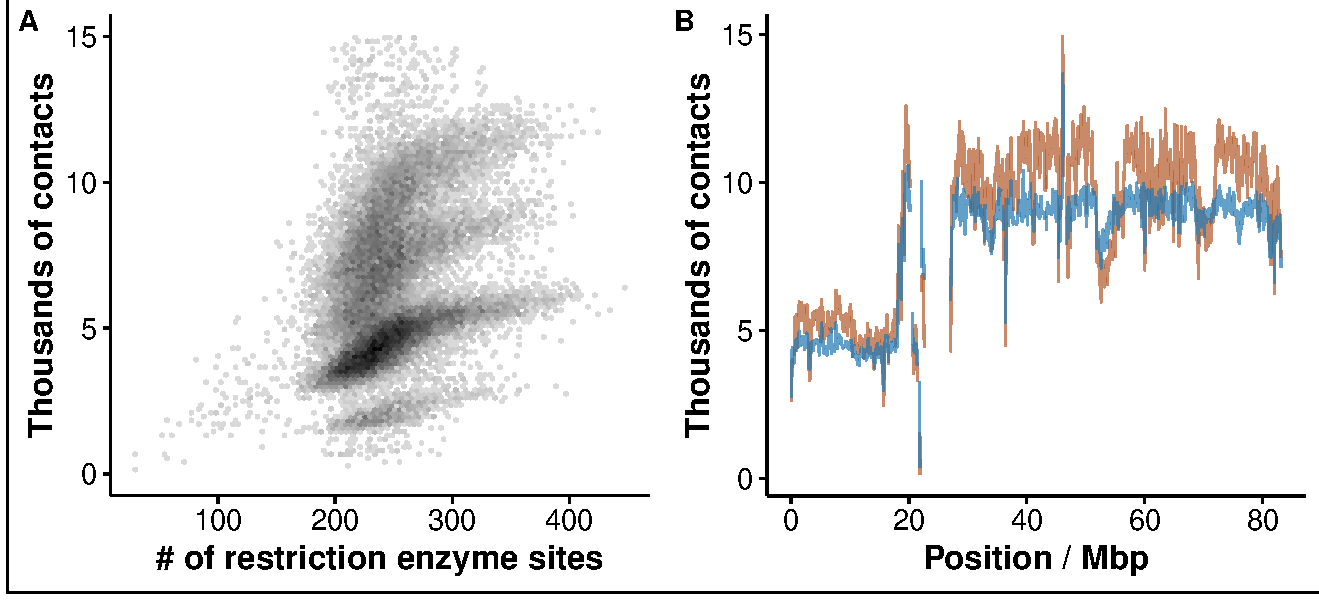
\includegraphics[width=.45\textwidth]{img/figure1.pdf}}
	\caption{
		A Non linear relationship between a genomic feature (number of restriction sites per bin) and the total number of contacts per bin for a T47D sample. B Total number of contacts per bin in chromosome 17 of a T47D sample. Raw (in brown, noisier) and corrected (in blue, more precise) data are depicted.
	}\label{fig:totals}
\end{figure}

\subsection{Data sources}

As an environment to test the bias correction, we gather a set of published \citep{ledily2014distinct,encode2012integrated,rao20143d,stadhouders2017transcription,lin2012global,dixon2012topological} and unpublished data from HiC experiments of different cell types and organisms. The details can be found in Table \ref{tab:samples}. Briefly, we used several experiments comprising T47D breast cancer cell lines (7 samples), K562 leukemia cell lines (4 samples), both with aberrant karyotypes, and mouse primary B (6 samples ) and ES (7 samples) cells, both with normal diploid karyotypes. The experiments used different protocols (\textit{i.e.} original HiC \citep{lieberman2009comprehensive} and in-situ HiC \citep{rao20143d}), different restriction enzymes (DpnII, HindIII, MboI and NcoI) and they were produced in distinct laboratories.

We also make use of array-based copy-number segmentation of the two cell lines obtained from COSMIC database \citep{forbes2010cosmic}.

\subsection{Data processing}

All data were processed though an in-house pipeline based on TADBit \citep{serra2016structural}. Briefly, after fastq quality control, paired reads were mapped against the corresponding reference genome (hg38 and mm10) taking into account the restriction enzyme motifs. Non-informative contacts were removed applying the following TADBit \citep{serra2016structural} filters: Self-circle, dangling-ends, error, extra dangling-end, duplicated and random-breaks. For more details, see methods of \cite{stadhouders2017transcription}. In addition, the pipeline is available, with minor modifications, in \cite{quilez2017managing} material.

We developed the routines contained in the \texttt{dryhic} R package to efficiently create sparse representations of contact matrices and further apply \textit{vanilla}, \textit{ice} and \textit{oned} corrections. \texttt{HiTC} \citep{servant2012hitc} and \texttt{HiCapp} \citep{wu2016computational} were used to get \textit{lgf} and \textit{caib} corrections respectively. All results are based on 100 Kbp resolution, although no major differences were found using different ones (data not shown).


\subsection{Total number of contacts as copy number proxy}

In euploid samples, we expect the coverage of a HiC experiment to be directly related to the number of copies (a duplicated region will show, on average, twice the number of contacts). An ilustrative example can be seen in Figure \ref{fig:copy_number}B. Given that our model is based on total number of contacts, which in turn is directly related to the number of copies, we reasoned that a preliminary test would be to check if the corrected number of contacts per bin ($ct_i = \sum_{i}{c_{ij}}$) reflects the copy number (as measured by an independent technique such as array-based copy-number segmentation) better than the alternatives.


\subsection{Sample comparison}

In order to test performance, we relied on pair-wise comparisons of contact matrices. However, there is little consensus on how to compare two HiC matrices. The simplest metric is the Spearman correlation applied to cis (intra-chromosomal) contacts up to a given distance (\textit{i.e.} 5 Mb). Though, the decay in the number of contacts with increasing genomic distance is the main driver of contact abundance and it could mask real differences between samples. This distance decay can be taken into account, for instance, computing the expected number of interactions given the genomic distance between any pair of loci. Thus, we can compare matrices in terms of observed over expected contacts, via the Pearson correlation (again focusing on a given distance range). Alternatively, we can compute the correlation per distance stratum and then obtain a stratum-adjusted correlation coefficient (SCC) as defined in \cite{yang2017hicrep}. Additionally, \cite{yan2017hicspector} proposed a reproducibility score based on the correlation between a set of the Laplacian matrix's eigenvectors (corresponding to the smallest eigenvalues) of the two experiments.

We defined three sets of samples: One with all T47D experiments plus two K562 samples, another with all K562 experiments plus two T47D samples and a third one comprising all mm10 samples (see Table \ref{tab:samples} for details). Given a set of experiments and a metric, we first computed all pair-wise combinations between experiments and then classified the comparisons according to the characteristics of each pair (\textit{i.e.} same / different cell types, same / different protocols, etc ...). 

To benchmark our method (\textbf{\textit{oned}}), we also test the performance of other alternatives. Three of them were based on the same implicit iterative correction \citep{imakaev2012iterative}: A first alternative computing one iteration (\textbf{\textit{vanilla}}), a second one iterating until convergence (\textbf{\textit{ice}}) and a third one using the chromosome adjusted iterative correction (\textbf{\textit{caib}}) \citep{wu2016computational}. The fourth one was inspired on the explicit bias correction originally presented by \cite{yaffe2011probabilistic}, but based on the local genomic features (\textbf{\textit{lgf}}) approach introduced by \cite{hu2012hicnorm} as implemented in \cite{servant2012hitc}.

Besides, we compared the raw matrices and used these comparisons as a baseline to present the gain / loss of correlation relative to the uncorrected data, thus allowing us to verify the effect of the bias correction procedure. The differences relative to the raw comparisons were estimated using a linear mixed model with the method as fixed effect and the chromosome as a random effect, and using the \texttt{lmer} function of the \texttt{lme4} R package \citep{bates2015lme4}.

In an attempt to further summarize the results, we reasoned that the correlation between unrelated samples (\textit{i.e} different cell types) should be lower than the correlation between related samples (\textit{i.e} same cell types), so we could re-interpret each correlation metric as a classifier score. Thus, we computed the receiver operating characteristic (ROC) curves and corresponding area under the curve (AUC) using the R \texttt{ROCR} package \citep{sing2005rocr}.

\end{methods}

\section{Results}

\subsection{Copy number}

Figure \ref{fig:totals}B shows the total number of corrected contacts along chromosme 17 of a T47D sample. Our correction approach presents a more stable and precise estimation of the copy number. Quantitatively (Figure \ref{fig:copy_number}), Pearson correlation with independent copy number data is high for both T47D and K562 cell lines (averages of 0.87 and 0.78 respectively), not only compared with raw data (averages of 0.74 and 0.63 respectively) but also with any of the alternative methods (averages ranging 0.39-0.68 and 0.30-0.53 respectively). Similar results were obtained using Spearman correlation (Supplementary Figure 2).


\begin{figure}
	\centerline{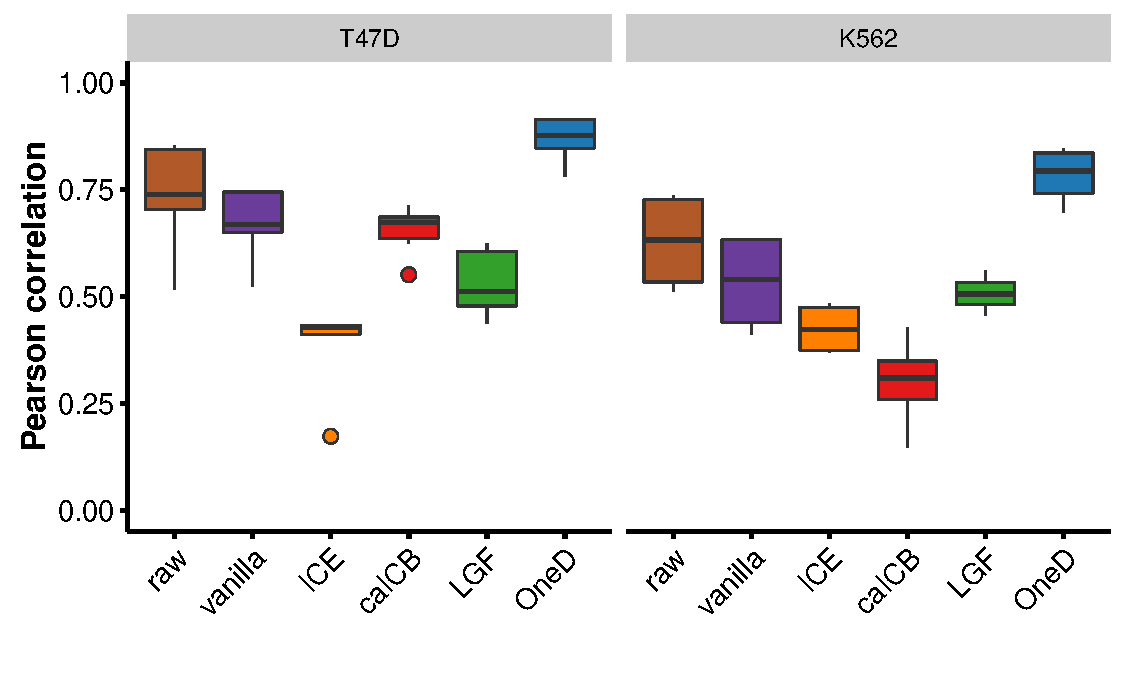
\includegraphics[width=.45\textwidth]{img/copy_number_figure2.pdf}}
	\caption{
		Pearson correlation between total number of contacts per bin and independent copy number estimation (COSMIC) for each of the methods compared. Left panel T47D breast cancer cell line, right panel K562 leukemia cell line. The new proposal (in blue) outperforms the rest of alternatives.
	}\label{fig:copy_number}
\end{figure}

\subsection{Samples with aberrant karyotypes}

Focusing on the Pearson correlation of observed over expected counts, methods based on the iterative correction (mainly \textit{ice} and \textit{caib} but also \textit{vanilla}) present the undesirable feature of higher correlations between unrelated samples than using raw data (top left panels of Figures \ref{fig:aberrant}A and \ref{fig:aberrant}C, Supplementary Figure 3). Among the comparisons of cells with the same type, \textit{oned} is the only method outperforming uncorrected data when comparing experiments using different protocols (top right panel of Figure \ref{fig:aberrant}A) and it is among the top performant when comparing experiments using the same protocol (rest of the panels in Figures \ref{fig:aberrant}A and \ref{fig:aberrant}C). Consequently, our proposal is the one that better discriminates unrelated samples form similar ones (as it can be seen in the ROC curves and AUCs of Figures \ref{fig:aberrant}B and D).

Complementary analysis using other metrics (Supplementary Figures 3, 4 and 5) yielded similar results. Notably, Spearman correlation of contacts presents the worst performance for all scenarios and seems to be a poor choice as a metric to compare HiC matrices.


\begin{figure}
	\centerline{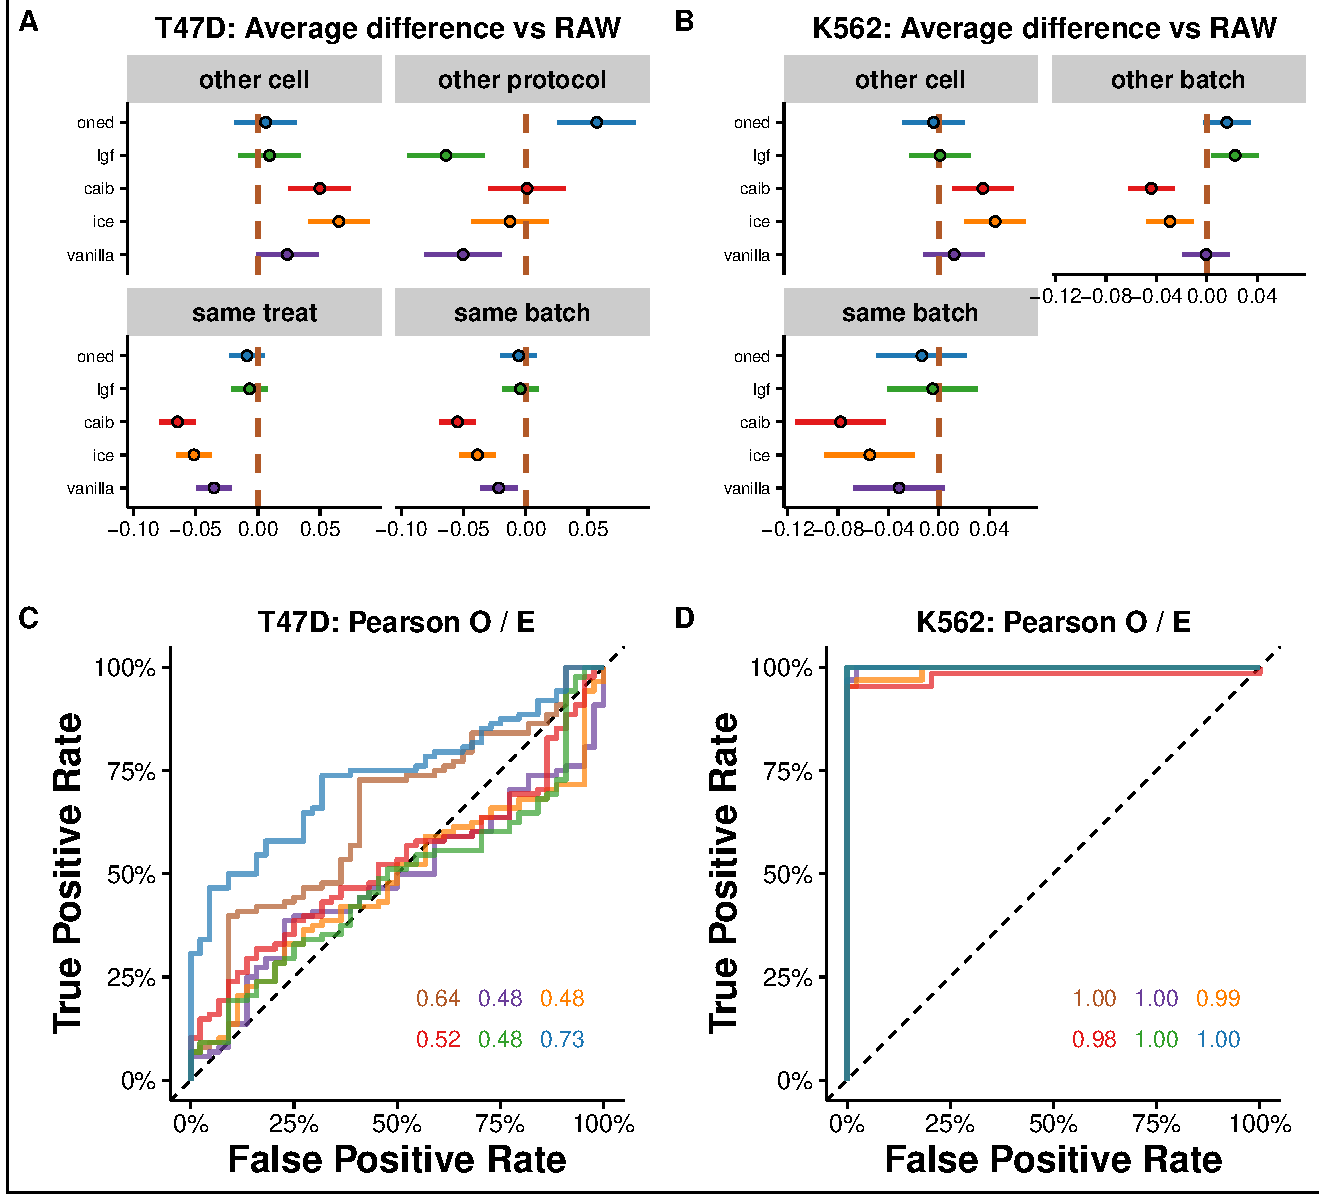
\includegraphics[width=.50\textwidth]{img/correlation_aberrant_figure3.pdf}}
	\caption{
		Results of the comparison between samples with aberrant karyotype. Left panels: Average difference and 95\% CI between each correction method (Y axis) and the raw data (brown dashed line) for T47D (A) and K562 (C) sets. Right panels: Corresponding ROC curves and AUCs for T47D (B) and K562 (D) sets. All results in this figure are based on Pearson correlations between the observed over expected counts. Our method increases reproducibility of similar samples while being able to discriminate different ones.
	}\label{fig:aberrant}
\end{figure}


\subsection{Samples with normal karyotypes}

Regarding cells with diploid genomes, we confirmed that our bias correction strategy also achieves good results in terms separation between unrelated and similar samples (Figure \ref{fig:normal} and Supplementary Figures 6 and 7), increasing the reproducibility across different experimental protocols for primary B and ES mouse cell samples. Again, Spearman correlation of contacts revealed as the worst metric.

\begin{figure}
	\centerline{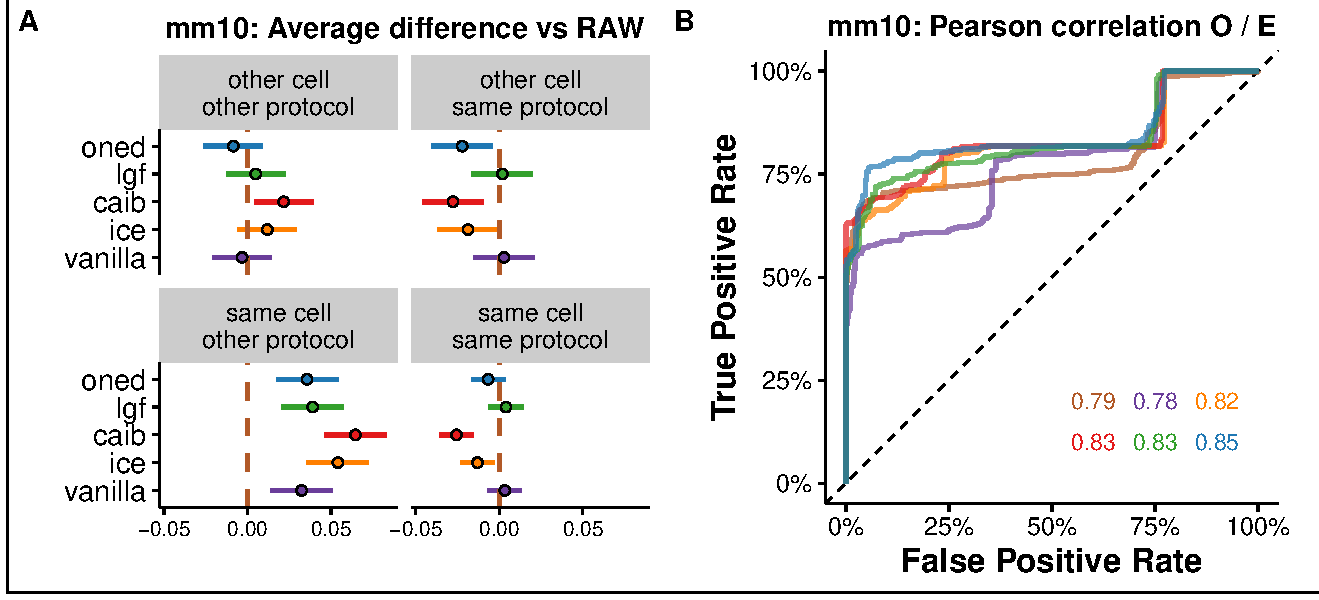
\includegraphics[width=.50\textwidth]{img/correlation_normal_figure4.pdf}}
	\caption{
		Results of the comparison between samples with normal karyotype. A Average difference and 95\% CI between each correction method (Y axis) and the raw data (brown dashed line) for the mm10 sets. B Corresponding ROC curves and AUCs. The introduced strategy does not under perform compared to the alternatives.
	}\label{fig:normal}
\end{figure}

\subsection{Computing resources}

One of the main reasons for the broad usage of the iterative correction \citep{imakaev2012iterative} is the easy and fast implementation, moreover compared to existing explicit methods \citep{servant2012hitc}. Our proposal uses only the total number of contacts per bin instead the full matrix for the model estimation. Thus, it achieves similar computing times that the fastest approaches (Figure \ref{fig:times} A). Yet it scales with increasing resolutions (decreasing bin size) (Figure \ref{fig:times} B).

\begin{figure}
	\centerline{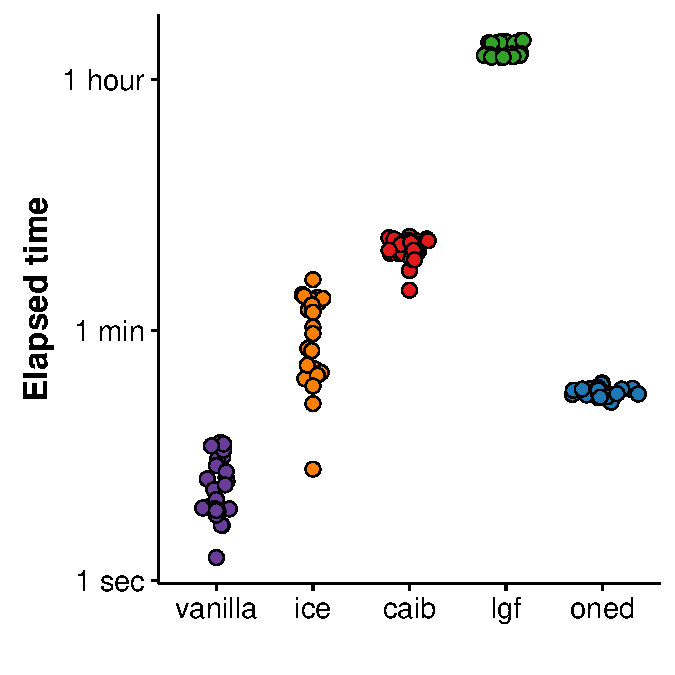
\includegraphics[width=.35\textwidth]{img/times_sina_figure5.pdf}}
	\caption{
		Computing time (Y axis, log scale) of all the bias correction methods used. Each dot corresponds to one sample. The only method faster than ours under performs in all sample comparisons.
	}\label{fig:times}
\end{figure}

\section{Discussion and Conclusions}


\section*{Acknowledgements}

We would like to thank all members of the four labs involved in the 4DGenome Synergy project for the fruitful discussions during project meetings. EV wants to acknowledge specially the members of Miguel Beato's lab for their insights during lab meetings.

\section*{Funding}

This work was supported by the Spanish Ministry of Economy and
Competitiveness, ‘Centro de Excelencia Severo Ochoa 2013-2017’,
SEV-2012-0208, ERC Synergy Grant 609989 (GF) and...
\vspace*{-12pt}

\bibliographystyle{natbib}
\bibliography{references}

\end{document}
